\documentclass{article}
\usepackage{amsmath, graphicx, amsfonts, caption, subfig, keyval}
\usepackage[numbers]{natbib}
\usepackage{xcolor}
\usepackage{hyperref}
\usepackage[boxruled,procnumbered, linesnumbered]{algorithm2e}
\usepackage[margin=0.5in]{geometry}
\usepackage{setspace}
\onehalfspacing
\usepackage{csquotes}

\captionsetup{justification=centering}
\newcommand{\R}{\mathbb{R}}
\newcommand{\Rr}{\mathcal{R}}
\newcommand{\D}{\mathcal{D}}
\newcommand{\C}{\mathcal{C}}
\newcommand{\X}{\mathcal{X}}
\DeclareMathOperator*{\argmin}{\arg\!\min}

\doublespacing
\makeatletter
\newcommand*{\toccontents}{\@starttoc{toc}}
\makeatother


% for the code & figure placement
%\usepackage{minted}
%\usemintedstyle{pastie}
\usepackage{float}
\floatplacement{figure}{H} % force figures to be placed always at defined position!

\begin{document}
\title{\Huge AM207 Final Project \\ \Large A dive into Bayesian Weather Modelling}
\singlespacing
\author{
  Victor Lei\\
           \small Institute for Applied Computational Science\\
	\small 52 Oxford Street\\
	\small Cambridge, MA\\
  \texttt{vlei@g.harvard.edu }
  \and
   Charles Liu\\
           \small Institute for Applied Computational Science\\
	\small 52 Oxford Street\\
	\small Cambridge, MA\\
  \texttt{cliu02@g.harvard.edu}
  \and
  Leonhard Spiegelberg\\
         \small Institute for Applied Computational Science\\
	\small 52 Oxford Street\\
	\small Cambridge, MA\\
 \texttt{spiegelberg@g.harvard.edu}
 \and
   Vinay Subbiah\\
         \small Institute for Applied Computational Science\\
	\small 52 Oxford Street\\
	\small Cambridge, MA\\
 \texttt{vinaysubbiah@g.harvard.edu}
}
\maketitle
\doublespacing
\begin{abstract}
Statistical weather modeling has a long tradition. In this project we apply different methods in a Bayesian context on historical weather data. Using a simplistic approach we implement and test Bayesian models based on a network topology (Bayesian Networks) and time series based models on weather measures like temperature, pressure or precipitation. In another modeling approach we investigate a hidden Markov model on weather events like rain, snow or fog. Statistical Inference based on these models has a wide range of possible applications. In this project we try to infer values for either missing data points (i.e. when measurements are not sufficient) or for missing stations / points.
\end{abstract}

\vfill
\singlespacing
\begin{center}
\bfseries\contentsname
\end{center}
\toccontents
\clearpage

\singlespacing
%%%%%%%%%%%%%%%%%%%%%%%%%%%%%%%%%%%%%%%%%%%%%%%%%%%%
%%-------------------------------                              Introduction                               -------------------------------%%
%%%%%%%%%%%%%%%%%%%%%%%%%%%%%%%%%%%%%%%%%%%%%%%%%%%%
\section{Introduction}
Traditional local and global weather modeling hugely relies on numerical simulations as well as statistical techniques. With the development and increasing popularity of Machine Learning algorithms in a Bayesian context, this project aims at serving as a study of techniques demonstrated along examples on how Bayesian techniques could be used for a data based approach in weather modeling.
\\
\\
Usually, weather data is collected at fixed weather stations that do not follow any particular pattern in terms of position or location. Hence, data is inherently spatially aware but not for every location is data available. Traditional approaches to infer missing data for specific locations rely either on numerical simulation results (and interpolating them) or on a local numerical simulation on a locally fine-grained grid. However, for many applications it is sufficient to use a statistical weather generator\cite{stochwg} which then can be used to infer a local distribution for weather parameters. One application of this could be for example to compute the risk of heavy rain for a location where no historical weather data is available. Another would be to actually use a statistical weather generator to construct initial boundary conditions of missing points that are then fed into a numerical model.
\\
\\
For this project we collected historical data of $18$ stations from $1960$-$2015$ around Boston from \url{wunderground.com}. 
\begin{figure}
\centering
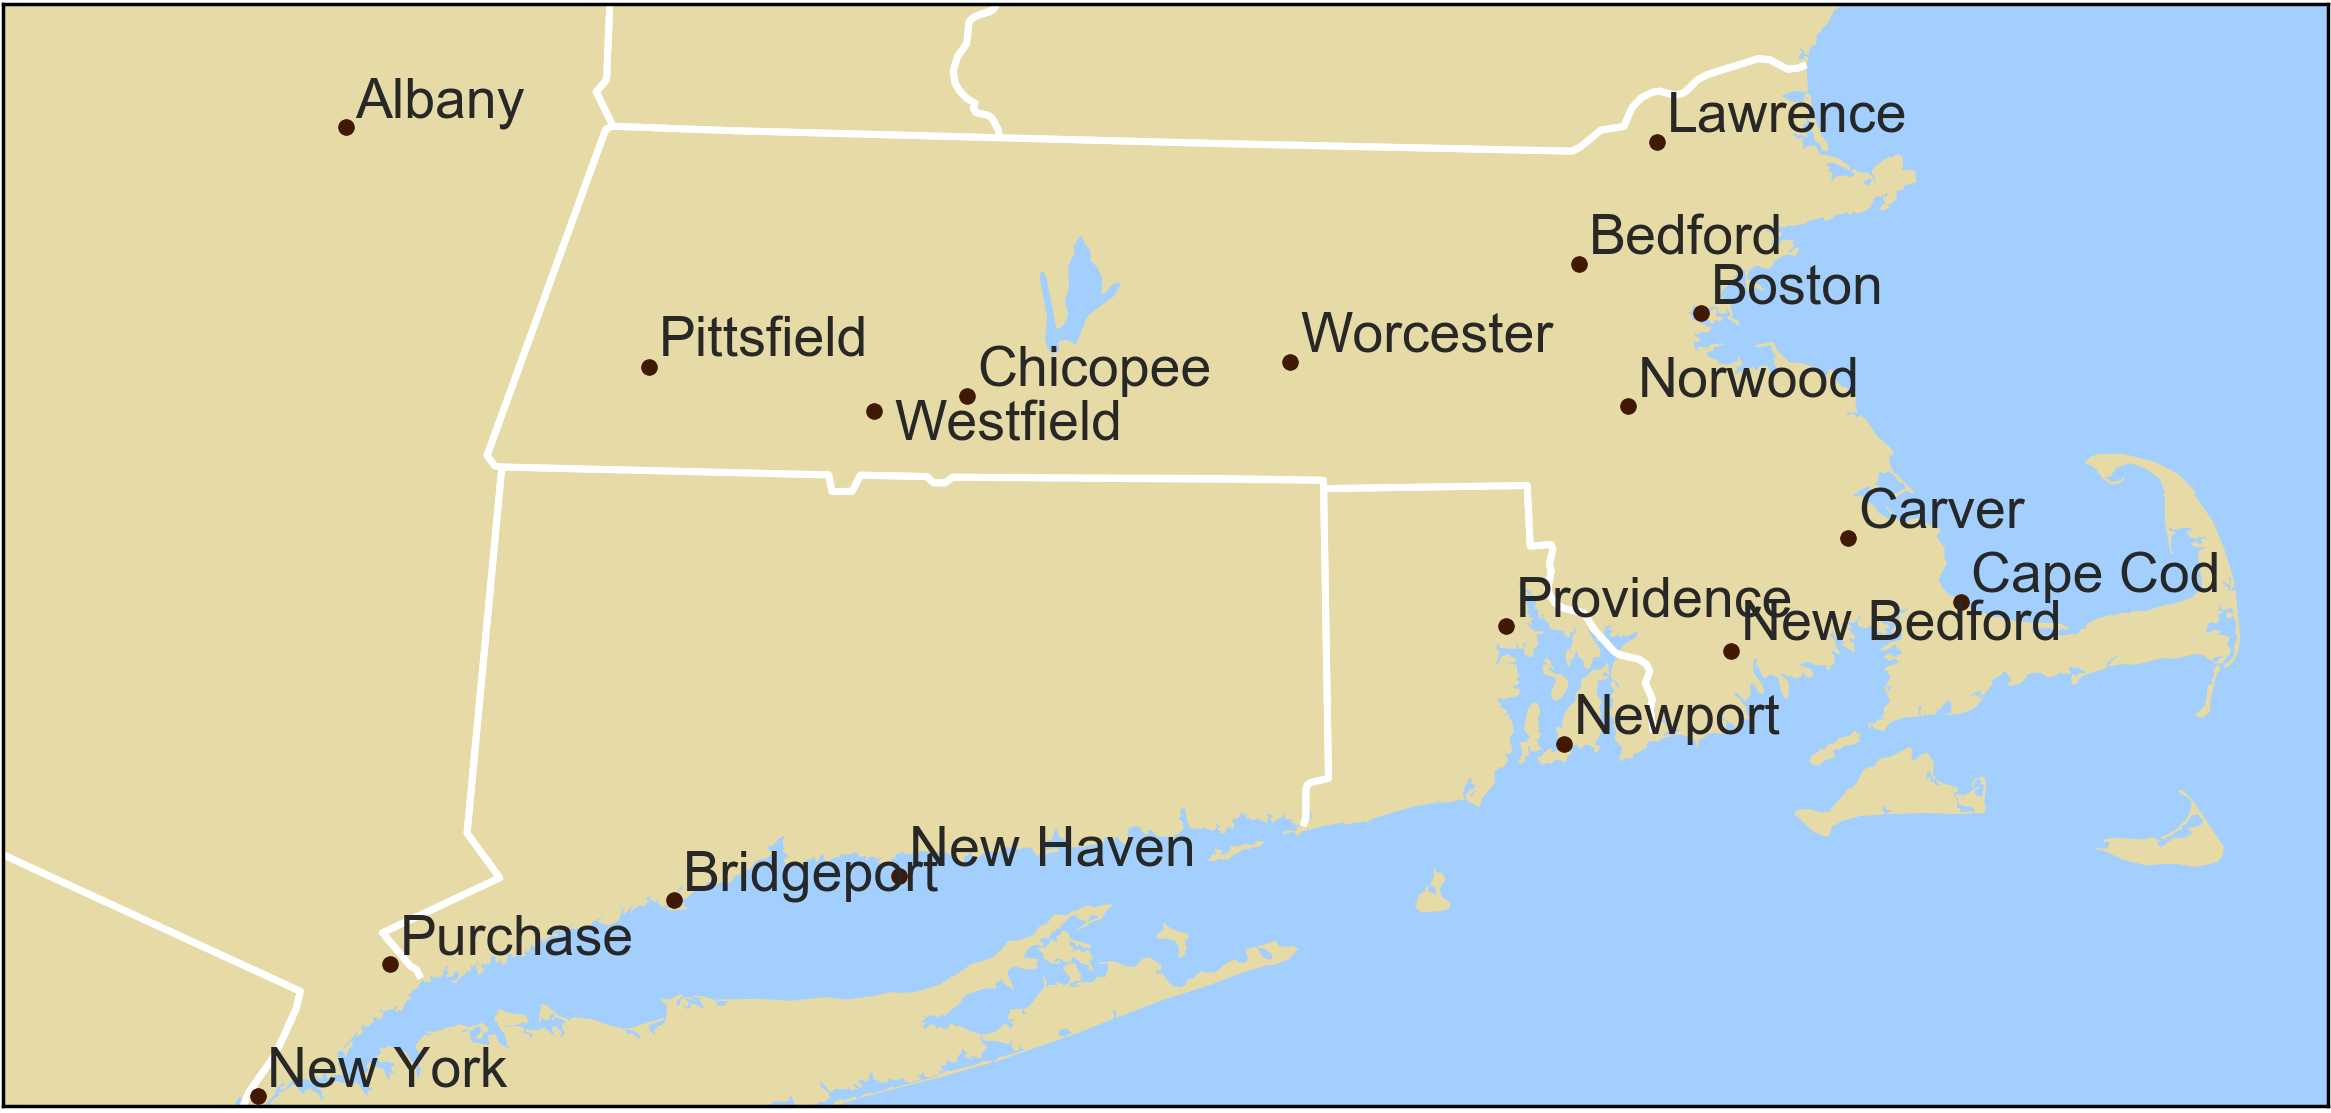
\includegraphics[scale=0.48]{../images/top_stations.png}
\caption{Illustration of the $18$ stations which data has been used for this project with weather stations being located next to airports.}
\end{figure}
Since historical weather data is usually hard to get or hidden behind paywalls, though we secured a decent amount of variables
% (Max TemperatureF,Mean TemperatureF,Min TemperatureF,Max Dew PointF,MeanDew PointF,Min DewpointF,Max Humidity, Mean Humidity, Min Humidity, Max Sea Level PressureIn, Mean Sea Level PressureIn, Min Sea Level PressureIn, Max VisibilityMiles, Mean VisibilityMiles, Min VisibilityMiles, Max Wind SpeedMPH, Mean Wind SpeedMPH, Max Gust SpeedMPH,PrecipitationIn, CloudCover, Events, WindDirDegrees)
we do not claim that our data base should be used for a real-world application. Instead, it serves more as a base for applying several techniques and investigating their feasibility. The first part of our study investigates the modeling of single weather measures demonstrated along precipitation whereas the second part focuses on a state-based approach for weather events.
\\
\label{sec:intro}
\section{Bayesian Networks}
Due to its spatial awareness, a hierarchical structure based on independence is a natural candidate to model a single weather measure. Bayesian Networks have been successfully applied to model precipitation by using a combination of historical weather data and numerical simulation data \cite{SpainBN}. 
\subsection{Network construction}
However, the question on how to construct the dependency graph which needs to be acyclic is non-trivial as it is a proven NP-hard problem. Thus, possible solutions often rely on greedy algorithms. In the context of weather modeling, dependency are usually inferred by a combination of manual dependencies obtained via domain knowledge and automated processing. As we do not possess any in-depth domain knowledge about weather dependencies we opted to push automatic network structure learning further by automating the whole process.\\
One of the most popular algorithms for structural learning of a Bayesian Network is the K2 algorithm. But to make it work, an initial ordering of the nodes (i.e. stations) is needed. 
\subsubsection{Initial Ordering}
We assume that stations with a fewer distance are more likely to be dependent than stations that are farther away. 
\begin{figure}
\centering
\begin{tabular}{cc}
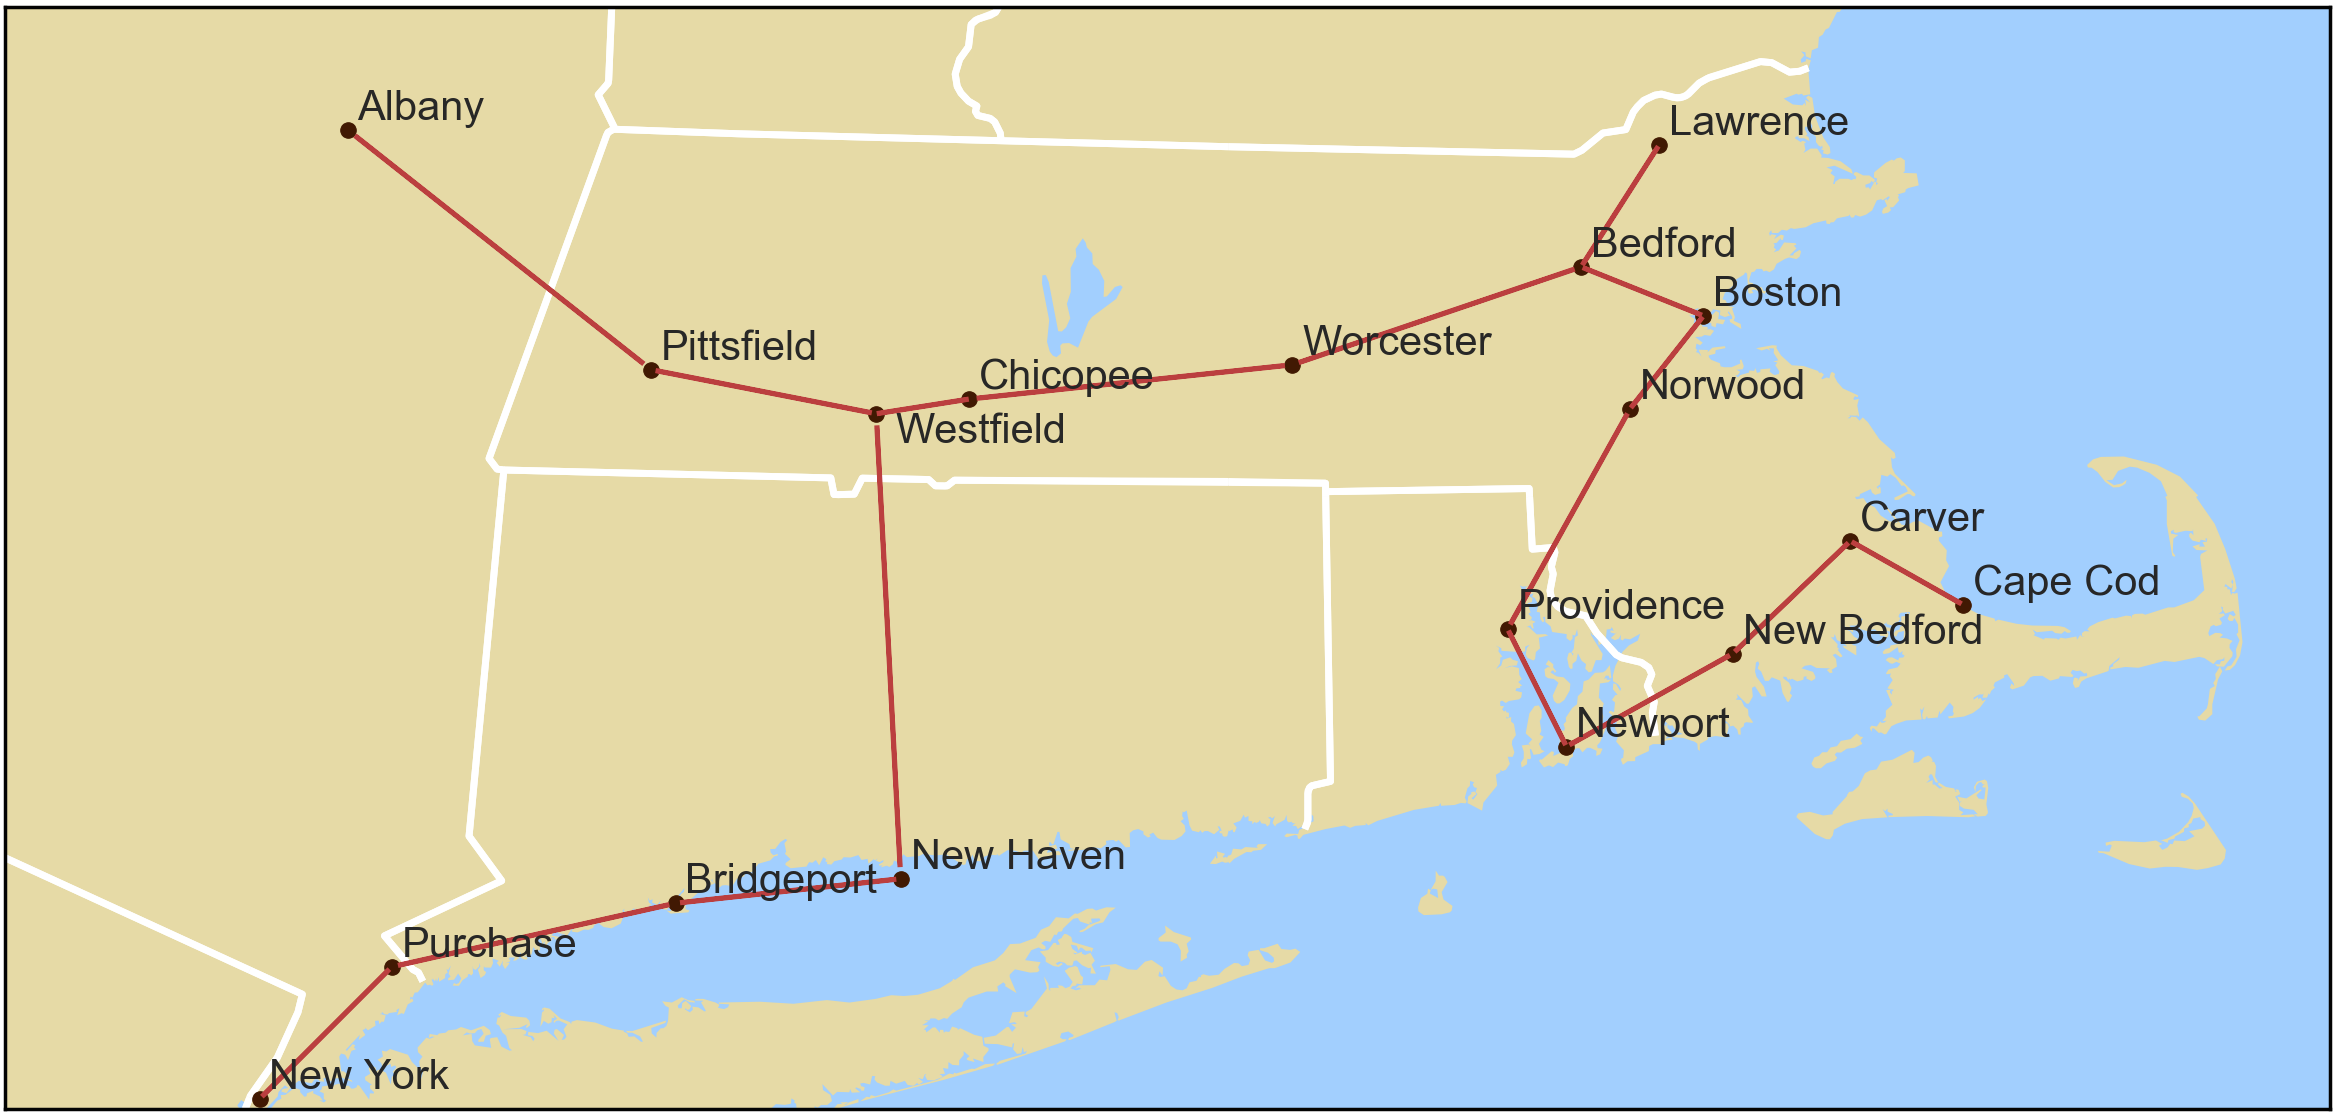
\includegraphics[scale=0.35]{../images/euclid.png} & 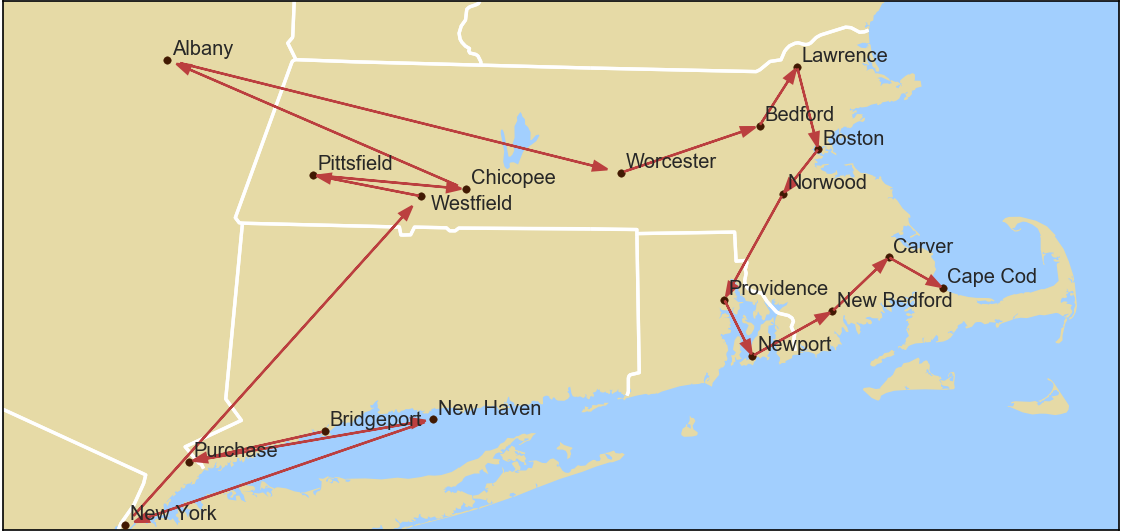
\includegraphics[scale=0.35]{../images/top.png} \\
a. Minimum Spanning tree with euclidean Distance & b. Topological Ordering
\end{tabular}
\caption{Construction of an initial node order. Arrows denote a child-parent relation.}
\label{fig:nodeordering}
\end{figure}
In a first step we construct a Minimum Spanning Tree (MST) with the euclidean distance used as edge weight (i.e. via Kruskal's algorithm\cite{kruskal}). Using this MST we select a node (typically one that has many neighbors in the MST) and perform a Breadth First Search (BFS) to obtain a topological ordering which is then used as input for the K2 algorithm. It should be noted that neither the MST nor the topological ordering are unique. Running the algorithm several times to obtain a plausible ordering is therefore strongly encouraged. Furthermore, we see this ansatz as a practical approach to get an initial dependency layout which can then be manually refined if needed (cf. \autoref{fig:nodeordering}).


\subsubsection{K2 + Simulated Annealing}
We created six buckets of precipitation levels - other than the first bucket which indicates no rain, the latter five were manually adjusted to have similar counts. K2 is a greedy algorithm based on our ordering heuristic. We define the probability that a node $i$ has parents $\pi_i$ as:
\begin{eqnarray*}
  f(i, \pi_i) &=& \prod\limits_{j=1}^{q_i} \frac{(r-1)!}{(N_{ij} + r - 1)!} \prod\limits_{k=1}^{r} \alpha_{ijk}!\\
  \text{where}\\
  q_i &:& |\{\text{Permutations of values for $\pi_i$}\}|\\
  r &:& |\{\text{Number of precipitation levels}\}|\\
  \alpha_{ijk} &:& |\{\text{node i with value $k$, parents $\pi_i$ with permutation j}\}|\\
  N_{ij} &:& \sum\limits_{k=1}^{r} \alpha_{ijk}
\end{eqnarray*}

Using this probability, we iterate through the ordering and for each node $i$ do the following:
\begin{displayquote}
\begin{enumerate}
  \item Calculate base probability with no parents
  \item Select the node preceding $i$ in the ordering that maximizes the probability
  \item If probability is greater than base probability:
    \begin{itemize}
      \item Update base probability
      \item Add node to list of parents
      \item Go back to 2
    \end{itemize}
  \item Otherwise return node's parents
\end{enumerate}
\end{displayquote}

\begin{figure}
\centering
\begin{tabular}{cc}
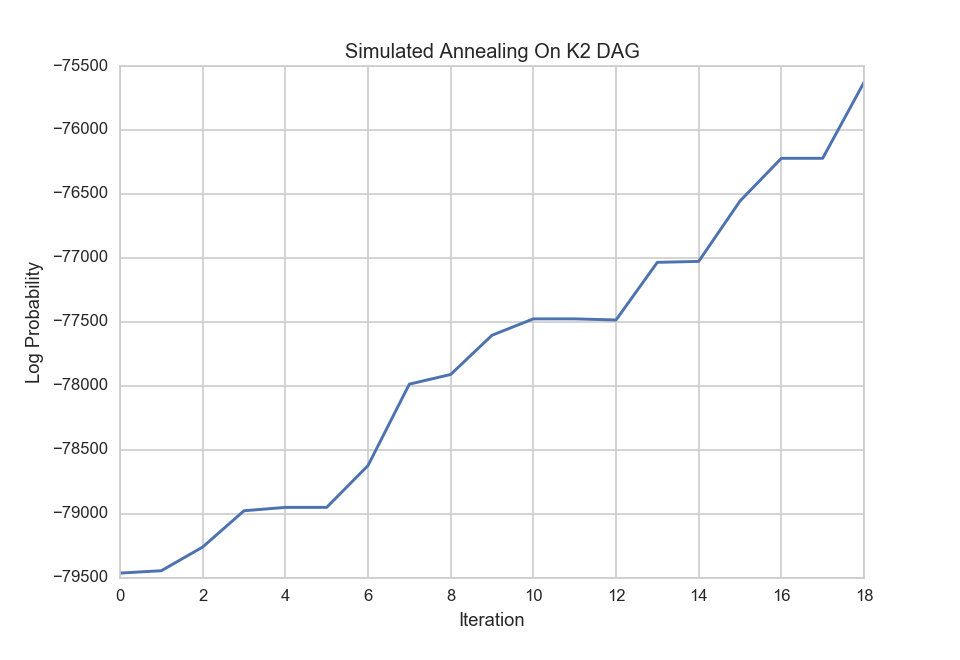
\includegraphics[scale=0.35]{../images/SA_BayesNet.png} & 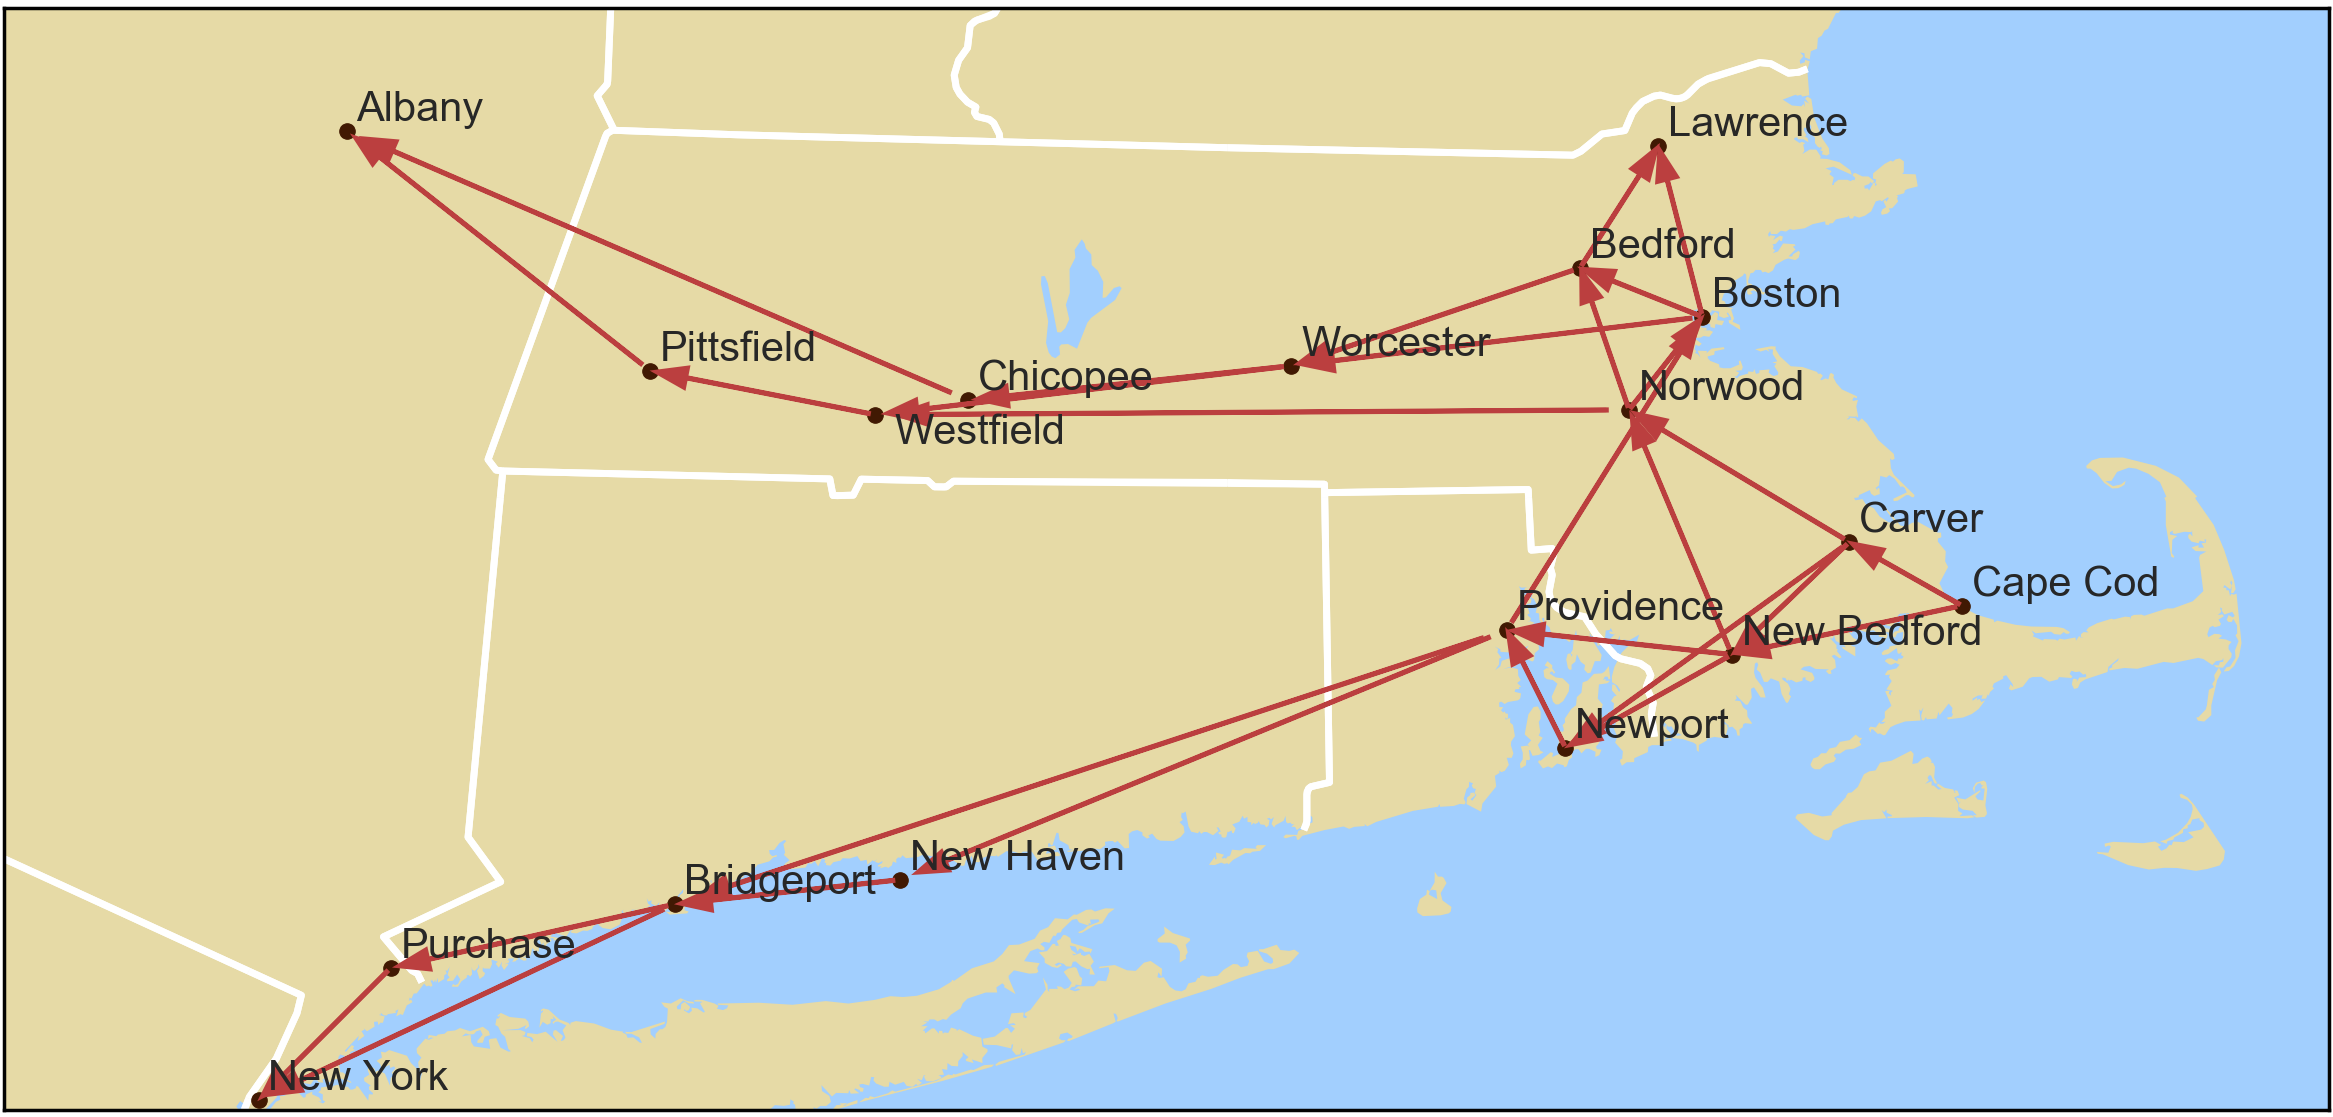
\includegraphics[scale=0.35]{../images/ordering.png} \\
a. Simulated Annealing & b. Final Bayesian Network
\end{tabular}
\caption{Simulating Annealing on K2 algorithm and resulting structure.}
\label{fig:bayesnet}
\end{figure}

As this algorithm is greedy, it has no guarantees on being optimal. We took the resulting structure from the K2 algorithm and ran Simulated Annealing, randomly selecting parents for a node based on temperature. Over 1000 iterations we saw only nine improvements, but the resulting dependency structure seems reasonable [cf. \autoref{fig:bayesnet}].

\subsection{Inference}
\subsubsection{Direct Sampling}
\begin{figure}
\centering
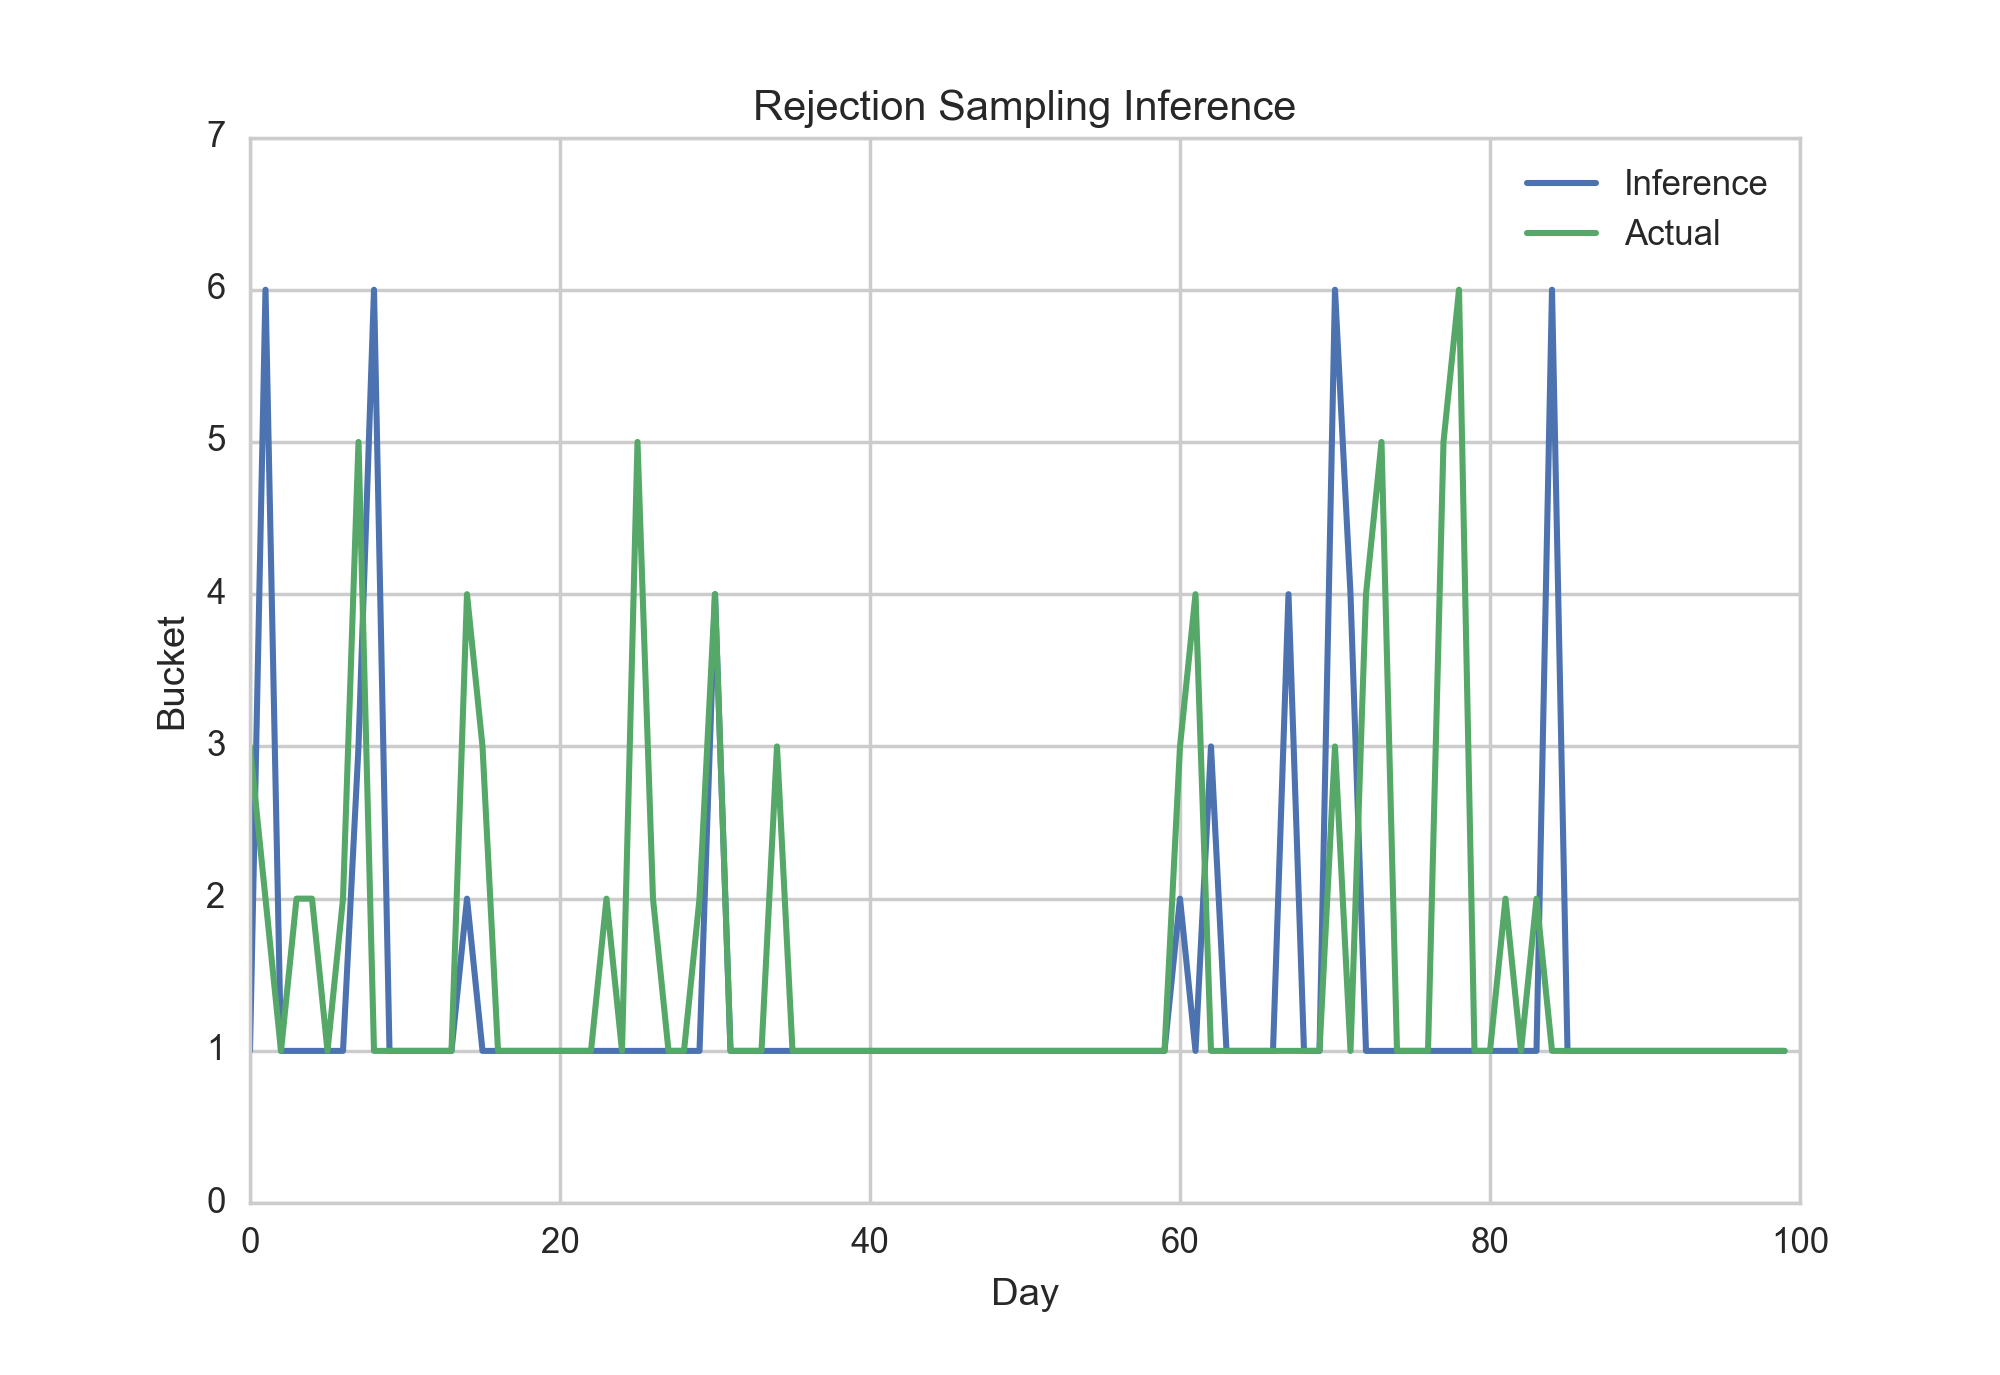
\includegraphics[scale=0.5]{../images/rej_samp.png}
\caption{Rejection Sampling For Inferring Boston Precipitation.}
\label{fig:rejsamp}
\end{figure}

We used rejection sampling as a simple method to infer historical precipitation levels. Using the empirical data, a sample is created by iterating through the node ordering and sampling from the conditional probability distribution based on the parent nodes. We tried to model the precipitation levels of Boston via it's parents in our network. For each historical data point we created many samples, rejecting those where the parents' precipitation levels didn't match with those from the historical data point. The resulting distribution was then sampled to obtain the precipitation level for Boston that day [cf. \autoref{fig:rejsamp}].


\subsubsection{Monte Carlo / Gibbs Sampling}
Another approach to sample the Bayesian Network is to use Gibbs Sampling. Let $X^{(t)} := \begin{bmatrix} X_1^{(t)} &  ... & X_n^{(t)} \end{bmatrix}^T$ a vector of random variables describing the current state of each of $n$ nodes at time $t$. Then we can sample a new state vector by picking randomly one $X_i^{(t)}$ and sampling a new representation of it by conditioning on the other variables, i.e. draw $X_i^{(t+1)} \sim \mathbb{P}(X_i^{(t)} \vert X_1^{(t)} , ..., X_{i-1}^{(t)},X_{i+1}^{(t)}, X_{n}^{(t)})$. For Bayesian networks we know that conditioning on $X_1^{(t)} , ..., X_{i-1}^{(t)},X_{i+1}^{(t)}, X_{n}^{(t)}$ is equal to conditioning on the parents, the children, and the parents of the children of $X_i$.The set of these nodes is also called the markov blanket of $X_i$ \cite{gibbsnips}. Repeating this process will eventually converge to the distribution as implied by the Bayesian Network's model (cf. \autoref{fig:gibbssampling}).
\begin{figure}
\centering
\begin{tabular}{cc}
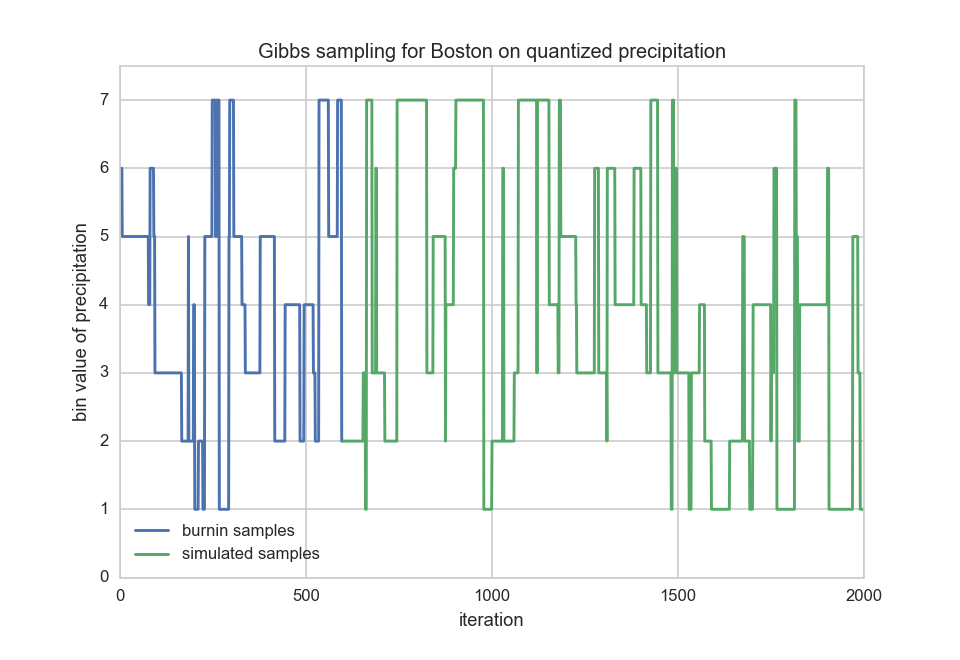
\includegraphics[scale=0.35]{../images/gibbs.png} & 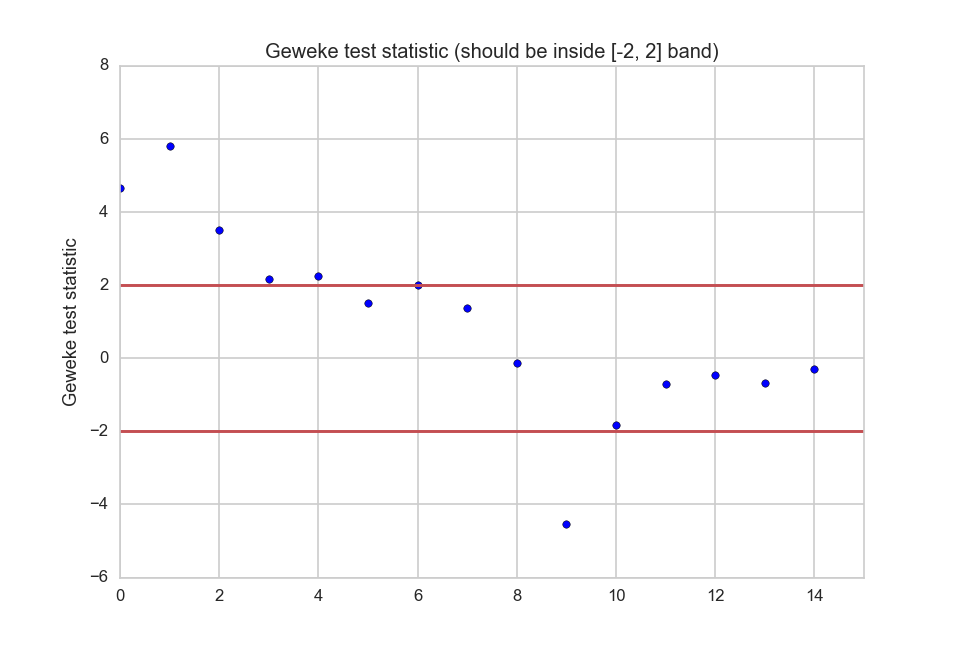
\includegraphics[scale=0.35]{../images/geweke.png} \\
a. Inference using Gibbs Sampling for Boston & b. Geweke test statistic
\end{tabular}
\caption{Exemplary stochastic precipitation generator for Boston using Gibbs Sampling. Due to complexity of data many samples are needed for convergence.}
\label{fig:gibbssampling}
\end{figure}

\subsection{Next steps}
The Bayesian Network assumes that weather properties for a particular region are derived from other local regions. While our model only relies on precipitation data, it can easily be extended to include models on atmospheric pressure and the like. The motivation for this would be to infer some properties of a region where weather data is hard to find - an ordering that ends on that region would then create its dependency structure. It can also be used for filling in missing historical data - in our case some regions such as Boston had nearly every data point between 1960 to 2015 (around 20K points), whereas others had far fewer. We found the intersection of common dates between all 18 regions was only around 5000 points, so one potential use case would be to look through the missing data and try to infer its precipitation levels through available data from the network.

\section{Bayesian Hierarchical Modeling of Rainfall Volume}
Rainfall models are typically focused on two issues: 
\begin{enumerate}
\item the probability of any rainfall; and
\item the volume of rainfall when it does rain.
\end{enumerate}
Here, we are focused on the second question. Traditional models for rainfall volume have found that the daily rainfall volume typically follows a Gamma distribution with shape parameter $\alpha$ and rate parameter $\frac{\alpha}{\mu}$ such that the expected volume of rainfall for each day is $\mu$. \cite{buishand}

Coe et al. \cite{coe} made the simplification that that the shape parameter for the Gamma distribution would remain constant, citing previous studies that made this same claim. Instead, they focused on the $\mu$ variable  which could vary over time by the generalized linear model $\mu = h( g(t) )$. $h$ is some known function like an exponential, and $g$ is some functional form that describes the variation in the mean rainfall volume over time, such as a polynomial or Fourier series. Based on these ideas, we make two contributions that extend the discussion from the paper: producing a two-period annual model for rainfall volume with a variable switching-point, and assessing whether the shape parameter remains constant using this two-period model as has been claimed in previous works.

\subsection{The case of New Bedford, MA}
\begin{figure}
\centering
\begin{tabular}{cc}
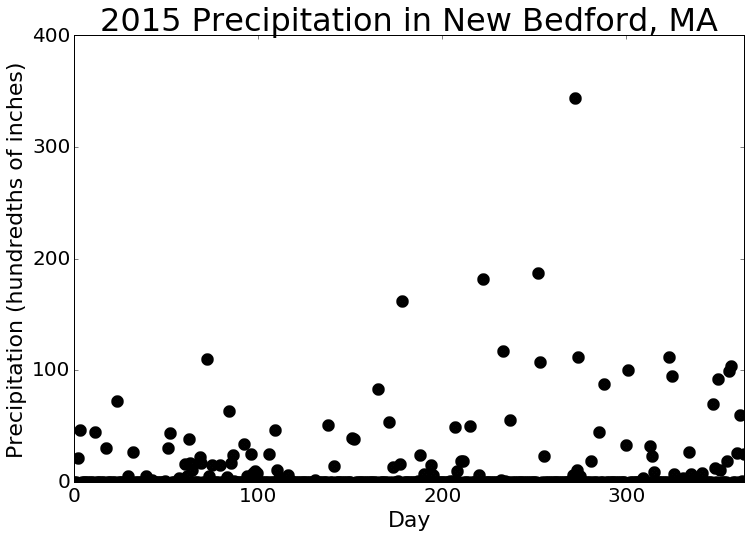
\includegraphics[scale=0.32]{../images/nbed_2015_rainfall_timeline.png} & 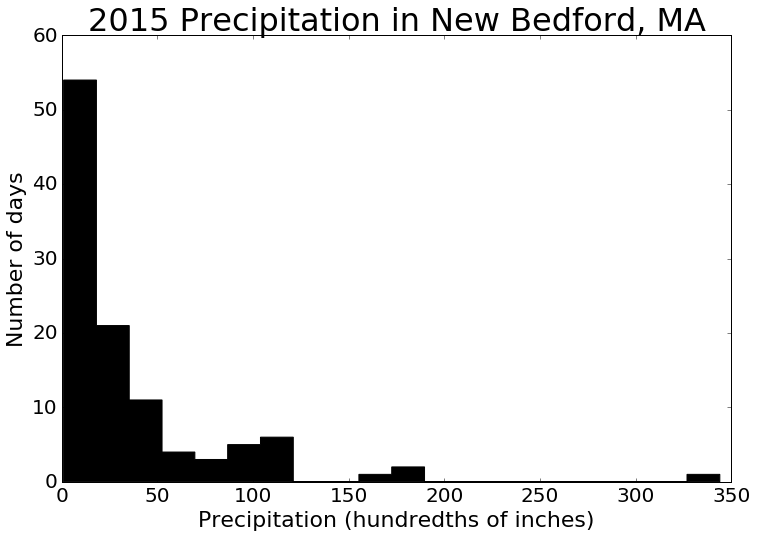
\includegraphics[scale=0.32]{../images/nbed_2015_rainfall_hist.png} \\
a. Precipitation over time & b. Histogram
\end{tabular}
\caption{Precipitation in New Bedford, MA during 2015.}
\label{fig:nbed2015_timeline}
\end{figure}

After analyzing plots of rainfall volume over time, we found at times, there appeared to be a lower volume of daily rainfall in the early part of the calendar year, followed by a marked increase towards the middle of the year.  We use the idea from Coe et al. of a time-varying $\mu$, but rather than fitting GLMs, we used the observation of this apparent increase in daily rainfall volume somewhere during the middle of the year to create a 'switching point' $s$ that breaks the annual rainfall volume into 2 separate Gamma distributions. We selected a rainy city that exhibited this behavior and focused on the 2015 data set as an example.

Logically, this idea makes sense since we might expect some seasons to produce a greater volume of rain than other seasons. We could also have done four switch points to coincide with the seasons, or 12 switching points to account for each month, but from the plots for New Bedford it appears two is sufficient to describe most of the variation and still retain a reasonable amount of data for the fitting process (there are around 100-120 rain days per year.) This may vary depending on the city and the year.

\subsection{Core intuition}
The key idea here is that the switching point segments the year so we retain some of the underlying time-based variability over the different seasons. Using pyMC, we can expose this switch point as another variable that we estimate on, and can then produce two separate models for rainfall volume. Compared to a fixed model that looks at the changing point for each season, this has the advantage of accounting for unusually short or long seasons, as is becoming increasingly common in recent years, plus we get uncertainty estimates for the switch point $s$.

This idea of a switching point is not necessarily going to apply well to all cities in all years; the climate is very variable and the underlying assumptions that exist for this model may not be present. However, as demonstrated here, we believe this technique of creating a switching point could be an interesting avenue used to explore and extend existing rainfall models.

\subsection{Results}
We fitted a standard Gamma distribution against the daily rainfall volume for the entire year, and then compared that to the results we obtained from fitting a two-period model with a variable switching point. We tried estimating both the shape and rate parameter separately, as well fixing the shape parameter across both models. In order to keep it brief, the results below are for fitting both the switching point, and the shape and rate parameters separately; further results are available in the notebook.

\begin{figure}
\centering
\begin{tabular}{cc}
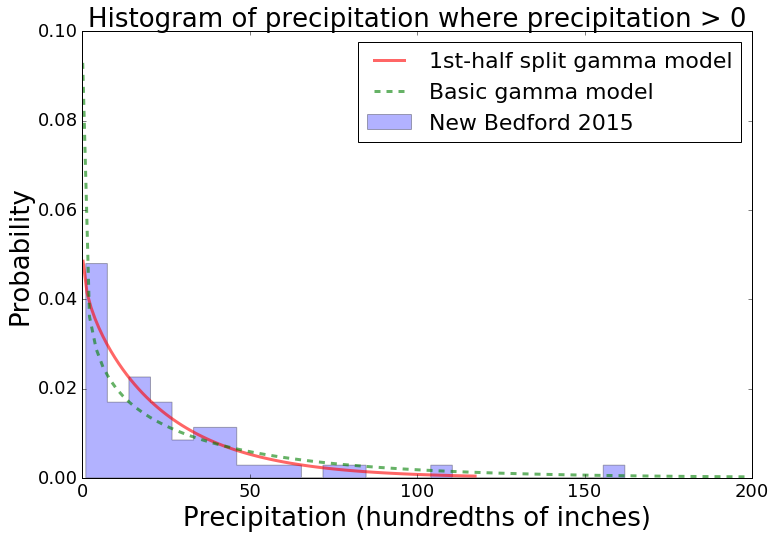
\includegraphics[scale=0.32]{../images/split_gamma_res_1.png} & 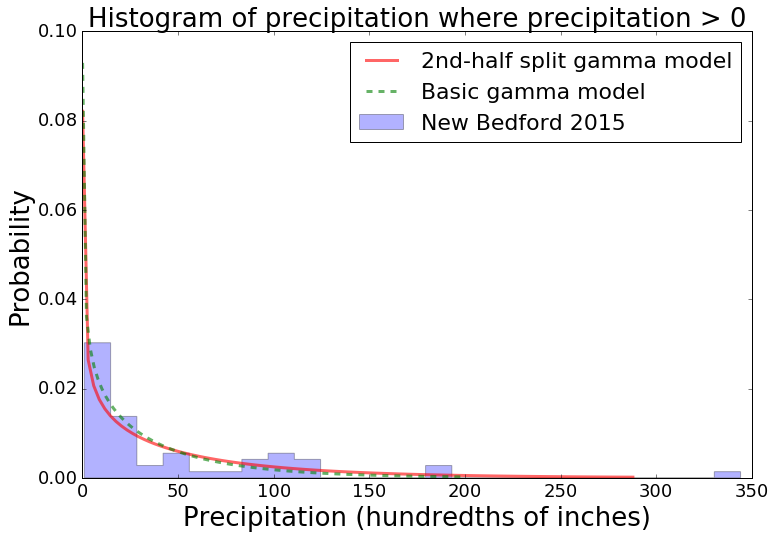
\includegraphics[scale=0.32]{../images/split_gamma_res_2.png} \\
a. 1st-half Gamma model & b. 2nd-half Gamma model
\end{tabular}
\caption{Fitting a 2-period Gamma model with variable switching point.}
\label{fig:split_gamma_res}
\end{figure}

As the results show, the Gamma model for the first part of the year does a better job of increasing the likelihood of lower rain volumes while decreasing the likelihood of higher rain volumes. The second part does the opposite, which is what we expect to see since it appears rainfall volume is higher during the second part of the year. So on the whole, we get a greater level of granularity and accuracy from creating this split model versus having a single model for the entire year.

The differences between the $\mu$ variable across the two Gamma models appear to be statistically significant, but the difference between the $\alpha$ variable appears to be only weakly significant. So the previous studies on the constant $\alpha$ variable are correct, at least in this instance.

\subsection{Next steps}
The key idea of the switching point can clearly be extended further, such as creating additional switching points. We can also make the 2-period model more robust by making the start and end points variable so that they do not need to coincide with the start and end of the calendar year; this would require an additional switching point. We might also consider the circumstances under which this model might work and when it might not, for example the geographical location of cities this would apply to, the types of climate in those cities, and which years.

\section{Hidden Markov Model}

Weather is often very hard to predict through purely statistical methods even when we have a sense of the weather measures. Nevertheless, we have attempted to model weather events based on weather measures using a second order Hidden Markov Model. This then provides a hierarchical framework through which to predict and study weather starting from Bayesian methods to model a specific weather measure like precipitation (as discussed above) all the way through to modeling and predicting specific weather events like Rain or Snow. Specifically, we are interested in seeing how well we can predict extreme weather events or other specific events like Fog days that have an adverse impact on people and society. In a similar study carried out by Betro, Bodini and Cossu \cite{Betro}, it has been demonstrated that HMMs are a reasonable model to attack this problem with the key underlying assumption that there exists discrete weather states corresponding to the hidden states of our model.  

\subsection{Data}

For our study, we have decided to focus on Boston, MA as we have reliable data going back more than $50$ years across a wide range of weather measures. We have $19$ discrete labels on our data representing weather events that correspond to a condensed $9$ hidden states in our model. This mapping was chosen to ensure each hidden state had a minimum number of data points for statistical analysis. The bucketing chosen also ensures that only neighboring events in terms of similarity were bucketed together. For example, Rain-Snow-Thunderstorm, Fog-Rain-Snow-Thunderstorm and Rain-Hail-Thunderstorm were all considered to simply be Thunderstorms. The observed states in our model correspond to 7 continuous real-valued weather measures like Mean Humidity, Mean Wind Speed etc. 

The model was trained on 50 years of data (1st Jan 1960 to 31st Dec 2010) and tested on the following five years (Jan 1st 2011 to Dec 31st 2015).

\subsection{Model}

The architecture of the model which is a second order Hidden Markov Model [cf. \autoref{fig:HMM_states_obs}]. Given the data available, our model does not require an expectation maximization framework to estimate the emission probabilities or transition probabilities. Instead, to model the emission probabilities, we modeled each of the observations as either a Gaussian distribution or a Log-normal distribution. We inferred the corresponding distribution parameters from the historical data. We then constructed a multivariate Gaussian representing the probability of a vector of observations corresponding to a particular hidden state. To model the transition probabilities, we simply counted the state transitions between the discrete weather events available in our labeled data. We also used a naive estimate of the initial state probability for our model. 
\\
\\
To infer the weather events on each day over our test period, we ran an extended Viterbi algorithm to infer the most probable sequence of hidden states given the observations over the five year test period. Using the recursive tracing approach, introduced by \citeauthor{He} \cite{He}, evaluating the maximum a posteriori estimation of the second order HMM is easily extendable to higher order models to improve the inference accuracy further.      
 
\begin{figure}
\centering            
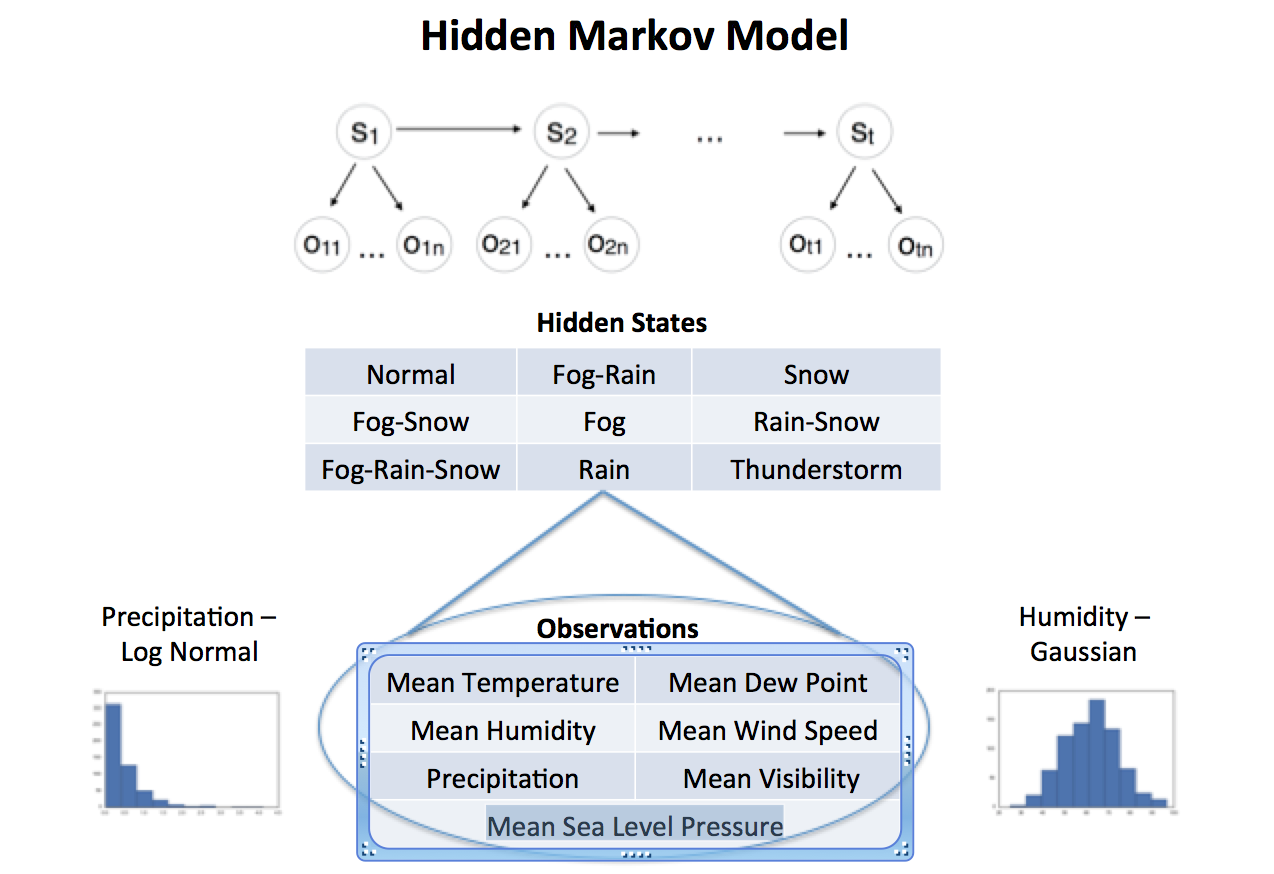
\includegraphics[scale=0.5]{../images/HMM_HS_O.png} 
\caption{Second order HMM with 9 hidden states and 7 observations}
\label{fig:HMM_states_obs}
\end{figure}

\subsection{Results}

Over the five year test period, the model had an overall accuracy of over $65\%$ [cf. \autoref{fig:HMM_results}]. Particularly, the model did well to infer extreme events like thunderstorms and specific events like Fog days as can been seen in \autoref{fig:HMM_results}. The model did less well on highly overlapping events like Rain, Rain-Snow or Fog-Snow. However, still considerably better than a na�ve baseline. Furthermore, even for the worst performing states, from an end-user standpoint, this is not as bad as it seems. In this problem, there is an inherent ordering of the hidden states, with some states being closer to each other than others. For example,  Rain-Snow, Rain and Fog-Rain-Snow are more similar to each other than to Fog days or Normal days which implies that such a misclassification is less impactful than would seem initially. The confusion matrix indicates the same and is discussed with further detail in the accompanying notebook.  

\begin{figure}
\centering            
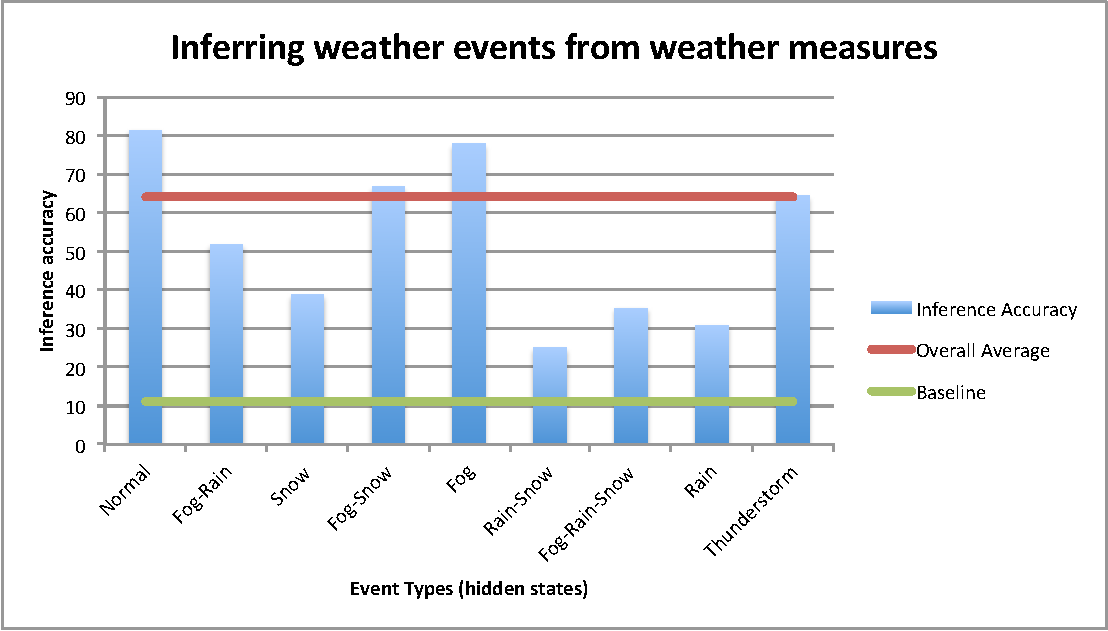
\includegraphics[scale=0.5]{../images/HMM_results.pdf} 
\caption{Inference accuracy over the five year test period}
\label{fig:HMM_results}
\end{figure}

\subsection{Next Steps}

Some extensions to the above model can also be studied further including the stationarity of the transition probabilities over the $50$ year training period and a possible third order model for improved inference. 
Also, as next steps, this model can be further extended by including more observation parameters that would express different aspects of the hidden states or more appropriate parameters like the max/min instead of the mean. Fundamentally, this analysis helps us infer weather events in places/times where we can't directly experience it as in the past/future, or on a different planet for which we only have weather measures. 










%% print out bib
\onehalfspacing
\bibliographystyle{plainnat}
\bibliography{bibliography}

\end{document}